\chapter{Portainer}
Docker wordt meestal via de command line gebruikt. Echter is het ook mogelijk om een UI te gebruiken voor het beheren van Docker. Dit kan door middel van Portainer.

\begin{figure}[H]
	\centering
	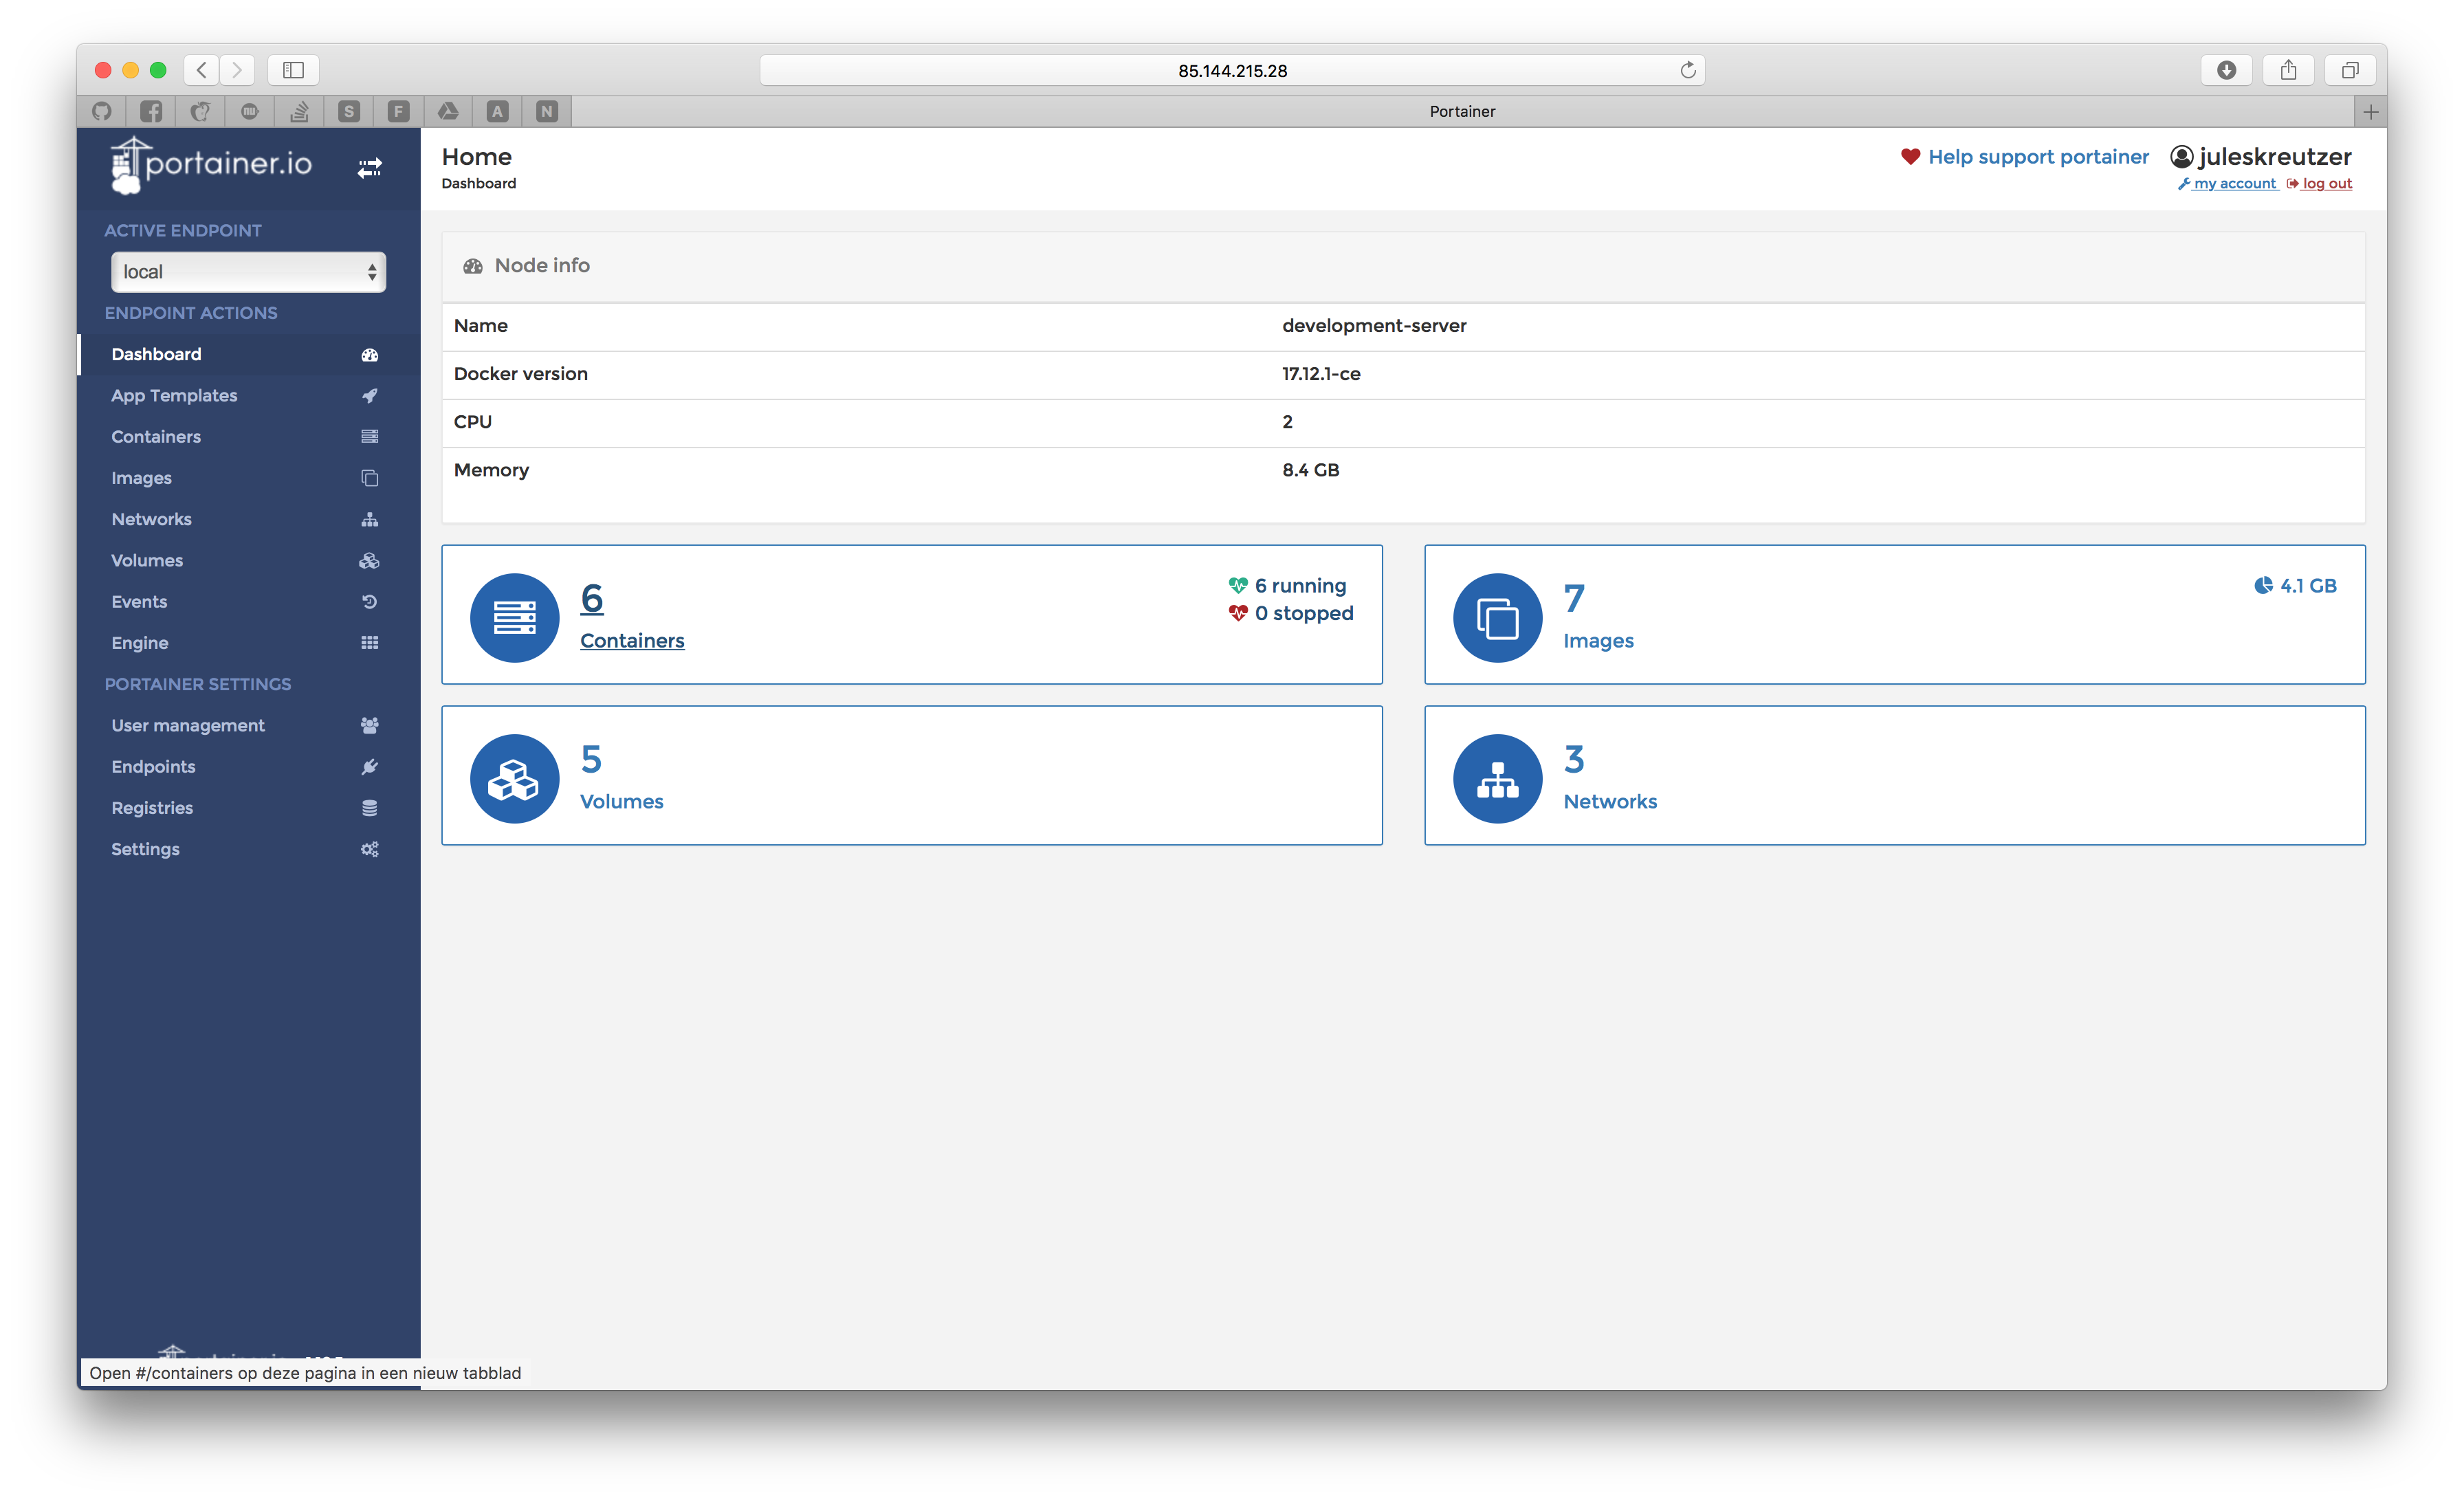
\includegraphics[width=0.95\textwidth]{img/PortainerDashboard.png}
	\caption{Het dashboard van Portainer, waarin weergegeven wordt dat er verschillende containers online zijn}
	\label{fig:PortainerDashboard}
\end{figure}

\section{Images}
Met de standaard instelling van Portainer zijn alle images die toegankelijk zijn op Docker hub en op de machine waar Portainer op draait beschikbaar. 
Wanneer een image vanuit docker hub lokaal is gepulled, zijn hier verschillende gegevens van beschikbaar: 
\begin{itemize}
	\setlength\itemsep{0em}
	\item Image details (id, omvang, build datum, ...)
	\item Dockerfile details (exposed ports, CMD, entry point, environment variabelen)
	\item Image layers
\end{itemize}

\section{Container}
Wanneer een image lokaal beschikbaar is gemaakt, kan in portainer een nieuwe docker container worden aangemaakt. Binnen deze docker container kunnen verschillende instellingen worden gedaan. Zo kun je namelijk een volume aan de container koppelen, verschillende poorten mappen zodat de container van buitenaf beschikbaar is, ... 
Daarnaast zijn er verschillende geavanceerde instellingen mogelijk. Hierin kan bijvoorbeeld een restart policy gemaakt worden. 

Bij het opzetten van de software ontwikkelstraat zijn er verschillende images met bijbehorende containers gebruikt. Deze worden in de komende hoofstukken uitgelegd.

